\documentclass[10pt,twocolumn]{article}
\usepackage[margin=0.72in]{geometry}
\usepackage{booktabs,graphicx,microtype,amsmath,amssymb,hyperref}
\usepackage[numbers,sort&compress]{natbib}
\newcommand{\model}{Qwen2.5-3B}
\title{A Readable but Not Cleanly Controllable ``Sounds Like AI'' Direction}
\author{Anonymous}\date{}
\begin{document}\maketitle
\begin{abstract}
Can a residual-stream direction separating human- from machine-written text causally control how machine-written a model sounds? We estimate paired mean-difference directions from 240 HC3 questions in base and instruction-tuned \model. A single projection almost perfectly separates 60 held-out pairs (AUROC 1.000 instruct; 0.998 base), remains useful beyond observable length, readability, and domain controls, and aligns across checkpoints (cosine 0.974). We intervene during instruction-model generation on 36 held-out questions. Moving two training standard deviations toward the machine side raises an older GPT-2 detector's mean machine probability by 0.127; moving away lowers it by 0.125. However, both confidence intervals include zero, equal-norm random directions cause similar shifts, and a second detector disagrees in magnitude. The largest apparently humanizing effect on an HC3-trained detector ($-0.441$) increases DistilGPT-2 perplexity by 8.82. The corpus direction is highly readable, but our controls do not support a distinct, quality-preserving causal ``AI-ness'' axis.
\end{abstract}

\section{Introduction}
Machine-generated text is often said to have a recognizable voice: polished structure, explicit signposting, and generic helpfulness. Activation-based detectors suggest that authorship is also represented internally. Recent work reports transferable human--machine linear probes \citep{quaremba2026linear,svdetect2026}, and sparse-autoencoder features can detect artificial text \citep{kuznetsov2025feature}. But readout does not imply control: a direction may bundle topic, length, fluency, or source artifacts, and adding any large vector can alter decoding.

We ask whether a paired human--AI direction changes two independent text detectors in the expected direction while preserving fluency and relevance, and more specifically than an equal-norm random vector. We also ask whether the readout exists in a pretrained base model or is created by instruction tuning. The answer is cautionary: the direction is nearly perfectly readable in both checkpoints, yet its causal effect is not consistently distinguishable from random steering. Strong detector changes on the negative side coincide with worse perplexity. This argues against identifying a high-AUROC probe direction with a clean generative control axis.

\section{Related Work}
HC3 introduced matched human and ChatGPT answers and neural baselines \citep{guo2023hc3}. DetectGPT uses probability curvature instead of supervised lexical cues \citep{mitchell2023detectgpt}, while GPT-2 release work supplied a RoBERTa detector used here as an out-of-era measure \citep{solaiman2019release}.

Activation addition shows that residual directions can influence behavior \citep{turner2023steering,panickssery2023steering}. Quaremba et al. recover a shared machine-text direction \citep{quaremba2026linear}; SV-Detect constructs per-layer human--AI vectors \citep{svdetect2026}; and Kuznetsov et al. analyze detection through sparse-autoencoder features \citep{kuznetsov2025feature}. These motivate, but do not settle, quality-controlled generation steering. The Assistant Axis \citep{lu2026assistant} identifies a steerable default-persona direction. We do not reconstruct that axis; base--instruct alignment provides only a limited test of whether chat tuning creates our direction.

\section{Method}
\paragraph{Data.} From HC3's five domains, we retain pairs whose first human and first ChatGPT answers exceed 80 characters, shuffle with seed 481516, and use 240 pairs to estimate directions and 60 disjoint pairs for evaluation. Matching by question reduces topic confounding. Texts are truncated to 256 tokens.

\paragraph{Readout.} At each depth $\ell$, we take the final non-padding token activation and estimate
\begin{equation}
v_\ell=\frac{\mathbb{E}[h_\ell(x_{AI})-h_\ell(x_H)]}{\|\mathbb{E}[h_\ell(x_{AI})-h_\ell(x_H)]\|_2}.
\end{equation}
The score is $h_\ell(x)^\top v_\ell$. We choose the layer with maximal training AUROC and report test AUROC. We repeat this for \model{} base and instruct. A descriptive confound model uses log word count, words per sentence, first-person and informal-word rates, mean word length, and domain one-hots, with and without the projection.

\paragraph{Intervention.} In the instruct model the selected layer is 30. At each decoding step we add $\alpha\sigma v_{30}$ to the final token, where $\sigma$ is the training projection standard deviation and $\alpha\in\{-2,-1,0,1,2\}$. For 36 held-out questions we generate up to 120 tokens at temperature 0.75 and top-$p$ 0.9, pairing seeds. Controls are a fixed equal-norm Gaussian random direction at $\alpha=\pm2$ and a prompt requesting natural human online prose.

\paragraph{Outcomes.} The primary score is the public RoBERTa GPT-2 detector \citep{solaiman2019release}. A second HC3-trained RoBERTa detector \citep{guo2023hc3} is less distribution-independent but tests agreement; its polarity is calibrated on 20 unused HC3 pairs. Quality safeguards are DistilGPT-2 perplexity and an MS MARCO MiniLM question--answer relevance logit. We also record length and repetition. We report paired mean differences, 95\% percentile bootstrap intervals (5,000 resamples), and Wilcoxon tests in released tables. Intervals are descriptive and uncorrected for multiplicity.

\section{Results}
\begin{figure}[t]
\centering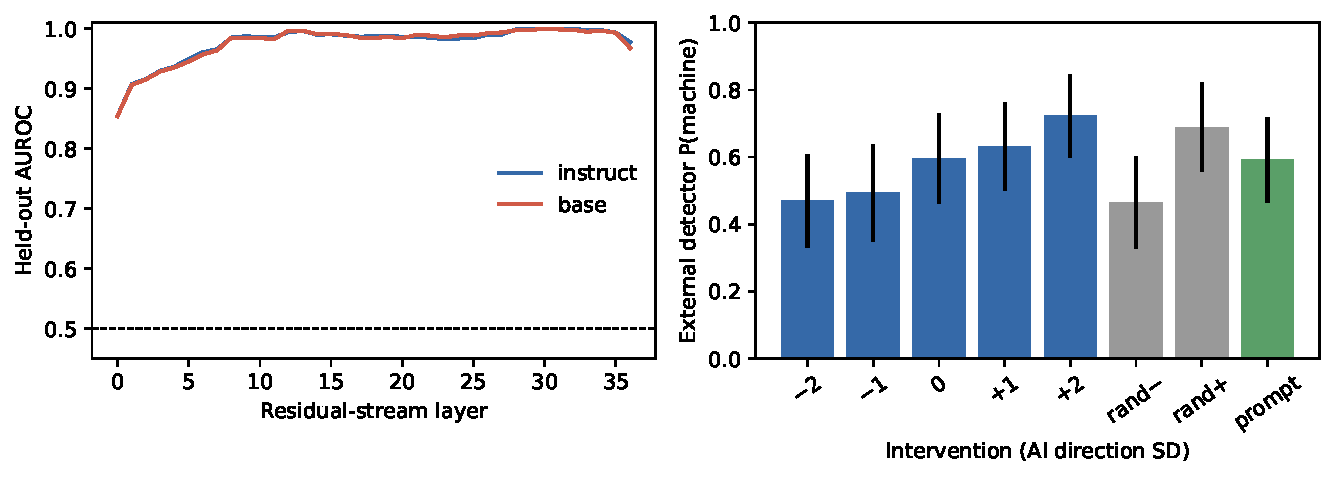
\includegraphics[width=\linewidth]{figures/main_results.pdf}
\caption{Left: held-out projection AUROC by layer. Right: mean external-detector probability; error bars show unpaired 95\% standard-error intervals for visualization.}
\label{fig:main}
\end{figure}

\subsection{Authorship is linearly readable}
Table~\ref{tab:readout} and Figure~\ref{fig:main} show near-ceiling separation. Training selection chooses layer 30 for instruct and 29 for base. The two layer-30 directions have cosine 0.974. Instruction tuning is therefore unnecessary for this readout and does not visibly amplify AUROC. Observable controls alone attain 0.845 AUROC; adding the instruct projection gives 1.000. This does not eliminate unmeasured corpus artifacts.

\begin{table}[t]\centering\small
\caption{Held-out matched-pair readout.}\label{tab:readout}
\begin{tabular}{lccc}\toprule
Checkpoint & Layer & Train & Test\\\midrule
Instruct & 30 & 0.999 & 1.000\\
Base & 29 & 0.999 & 0.998\\\bottomrule
\end{tabular}\end{table}

\subsection{Steering moves detectors, but not specifically}
Table~\ref{tab:causal} gives paired effects. On the older detector, fitted and random directions have nearly the same signed effect. Directly subtracting random-control effects from fitted effects gives 0.006 [${-0.186},0.196$] at $-2$ and 0.033 [${-0.118},0.189$] at $+2$.

The HC3 detector gives a large fitted-direction effect at $-2$ ($-0.441$), exceeding random steering by $-0.361$ [${-0.540},{-0.186}$]. Yet this condition increases perplexity by 8.82, 5.52 more than the random control [2.45, 8.61], so it does not establish quality-preserving humanization. The prompt-only control changes old-detector probability by $-0.003$ and raises perplexity by 4.24.

\begin{table*}[t]\centering\small
\caption{Paired change from baseline (95\% bootstrap interval), $n=36$. Detector columns are machine probability; higher relevance is better.}\label{tab:causal}
\begin{tabular}{lrrrr}\toprule
Condition & GPT-2 detector & HC3 detector & Perplexity & Relevance\\\midrule
AI direction $-2$ & $-0.125$ [$-0.313$, $0.068$] & $-0.441$ [$-0.593$, $-0.294$] & $+8.82$ [$5.52$, $12.11$] & $-0.10$ [$-1.22$, $1.01$]\\
Random $-2$ & $-0.131$ [$-0.293$, $0.034$] & $-0.080$ [$-0.180$, $0.008$] & $+3.30$ [$0.64$, $6.07$] & $+0.94$ [$0.07$, $1.88$]\\
AI direction $+2$ & $+0.127$ [$-0.036$, $0.279$] & $+0.023$ [$-0.045$, $0.103$] & $-0.48$ [$-2.57$, $1.59$] & $+1.45$ [$0.37$, $2.53$]\\
Random $+2$ & $+0.093$ [$-0.069$, $0.257$] & $+0.036$ [$-0.016$, $0.112$] & $+1.65$ [$-0.36$, $3.70$] & $+1.08$ [$0.32$, $1.93$]\\
Human prompt & $-0.003$ [$-0.172$, $0.169$] & $-0.139$ [$-0.261$, $-0.029$] & $+4.24$ [$1.61$, $6.88$] & $+0.54$ [$-0.30$, $1.37$]\\\bottomrule
\end{tabular}\end{table*}

Mean lengths remain tightly clustered (96.9--100.1 words). At $+2$, repetition rises from 0.301 to 0.327; random $+2$ reaches 0.319. Both target and random interventions can shift surface statistics and relevance, consistent with nonspecific perturbation.

\section{Discussion}
The experiment separates three claims. Authorship-correlated information is available: strongly supported. A matched mean difference affects generated text: weakly supported, because detector means move monotonically. The vector is a distinct, quality-preserving ``AI-ness'' controller: not supported. Random steering explains much of the old-detector movement, detectors disagree, and the strongest negative effect trades off against perplexity.

Base--instruct similarity disfavors a purely instruction-tuned persona explanation but does not prove distinction from the Assistant Axis. Related checkpoints share representations; a direct within-model comparison against a reconstructed persona axis is needed.

\section{Limitations and Ethics}
We use one 3B family, one corpus, one pooling position, 36 prompts, and one random direction. HC3 human answers differ stylistically from ChatGPT answers despite topic matching. One detector is old and the other is trained on HC3; neither measures perceived authorship directly. Perplexity and retrieval relevance incompletely proxy coherence and factuality. A planned API style judge could not run because both supplied endpoints rejected authentication; no judge scores are reported. We do not test formal transformations, cross-generator transfer, adversarial robustness, or the Assistant Axis directly. Multiple uncorrected comparisons make this exploratory.

Steering toward human detector scores could aid evasion. We emphasize that detector scores are unreliable under intervention. The negative specificity result cautions against treating internal projections as authorship evidence.

\section{Conclusion}
Human versus ChatGPT text is almost perfectly separable in both base and instruction-tuned residual streams. Nevertheless, adding that direction does not yield a clean ``sounds like AI'' control. Equal-norm random steering often shifts detectors similarly, and the strongest humanizing score change degrades perplexity. Linear readability is insufficient evidence of a causal, semantically distinct style axis.

\bibliographystyle{plainnat}\bibliography{references}
\end{document}
